\documentclass[conference]{IEEEtran}
\IEEEoverridecommandlockouts
% The preceding line is only needed to identify funding in the first footnote. If that is unneeded, please comment it out.
\usepackage{cite}
\usepackage{amsmath,amssymb,amsfonts}
\usepackage{algorithmic}
\usepackage{graphicx}
\usepackage{textcomp}
\usepackage{xcolor}
\def\BibTeX{{\rm B\kern-.05em{\sc i\kern-.025em b}\kern-.08em
    T\kern-.1667em\lower.7ex\hbox{E}\kern-.125emX}}
\begin{document}

\title{Better categorization of white blood cells by utilizing ResNet50V2 in the
4B-AdditionNet-based CNN network and ant colony optimization workflow\\
{\footnotesize \textsuperscript{*}Note: This paper is the result of a research practice course handout, the results are made up}
\thanks{Identify applicable funding agency here. If none, delete this.}
}

\author{\IEEEauthorblockN{4\textsuperscript{th} Bustya Balázs}
\IEEEauthorblockA{\textit{Eötvös Loránd University} \\
\textit{Faculty of Informatics}\\
Budapest, Hungary}
\and
\IEEEauthorblockN{4\textsuperscript{th} Csizmadia Árpád}
\IEEEauthorblockA{\textit{Eötvös Loránd University} \\
\textit{Faculty of Informatics}\\
Budapest, Hungary}
\and
\IEEEauthorblockN{4\textsuperscript{th} Nagy Norbert Botond}
\IEEEauthorblockA{\textit{Eötvös Loránd University} \\
\textit{Faculty of Informatics}\\
Budapest, Hungary}
\and
\IEEEauthorblockN{4\textsuperscript{th} Novák-Schwartz József}
\IEEEauthorblockA{\textit{Eötvös Loránd University)} \\
\textit{Faculty of Informatics}\\
Budapest, Hungary}
}

\maketitle

\begin{abstract}
    White blood cells, WBCs for short, are an essential component of the human immune system. These cells are our body’s
    first line of defense against infections and diseases caused by bacteria, viruses, and fungi, as well as abnormal and external
    substances that may enter the bloodstream. A wrong WBC count can signify dangerous viral infections, autoimmune disorders,
    cancer, sarcoidosis, aplastic anemia, leukemia, tuberculosis, etc. A lot of these diseases and disorders can be extremely painful
    and often result in death. Leukemia is among the more common types of blood cancer and when left undetected leads to
    death. An early diagnosis is necessary which is possible by looking at the shapes and determining the numbers of young
    and immature WBCs to see if they are normal or not. Performing this task manually is a cumbersome, expensive, and timeconsuming process for hematologists, and therefore computer-aided systems have been developed to help with this problem.
    This paper proposes an improved method of classification of WBCs utilizing a combination of preprocessing, convolutional
    neural networks (CNNs), feature selection algorithms, and classifiers. In preprocessing, contrast-limited adaptive histogram
    equalization (CLAHE) is applied to the input images. A CNN is designed and trained to be used for feature extraction
    along with ResNet50 and EfficientNetB0 networks. Ant colony optimization is used to select the best features which are
    then serially fused and passed onto classifiers such as support vector machine (SVM) and quadratic discriminant analysis
    (QDA) for classification. The classification accuracy achieved on the Blood Cell Images dataset is 98.44\%, which shows the
    robustness of the proposed work.
\end{abstract}

\begin{IEEEkeywords}
White blood cells · CNN · Classification · Preprocessing · Fusion · Selection
\end{IEEEkeywords}

\section{Introduction}
This document is a model and instructions for \LaTeX.
Please observe the conference page limits. 



The amount of blood in the human body can depend on a few factors, like your sex, how much you weigh, and even where you live, but generally equivalent to 7\% of the body weight. The amount of blood in the human body differs based on where you live. For example, people who live at higher altitudes usually have more blood because there isn’t as much oxygen at lower altitudes. The main component of the blood is plasma, which takes up 55\% of it.
The plasma allows the blood to flow freely throughout the entire body inside blood vessels. Based on different attributes of the blood’s cellular components, like colour, size, texture, composition and shape, they are separated into three cell types: erythrocytes also known as Red Blood Cells (RBC), leukocytes (White Blood Cells) and thrombocytes. Observing these molecules under the microscope, they have distinct shapes and sizes, WBCs being the larger ones due to the presence of nuclei and cytoplasm inside them. 
Based on these features WBC are further divided into two types: granulocytes and agranulocytes. 
Granulocytes are the most common WBC types defined by the granules inside their cytoplasm. The granulocytes, if dyed, can be categorized into four subtypes. These types differ in the colour of the granule stains inside the cytoplasm. The four cell types are neutrophils, eosinophils, basophils, and mast cells. The other type of WBC are agranulocytes that don't have granules in their cytoplasm and are further categorized into lymphocytes and monocytes.

%figure about WBC cells

A sample of 1 µl of human blood sample contains between 4000 and 11000 WBC. The distribution of different WBC types are the followings: neutrophils between 40\% and 70\%, lymphocytes between 20\% and 45\%, monocytes between 2\% and 10\%, eosinophils between 1\% and 6\% and basophils under 1\%. Although basophils make up less than 1\% of the blood, they play an important role in the health of humans. Any minor imbalance can cause serious health issues, e.g., leukemia, 
% https://www.sciencedirect.com/science/article/pii/S0169260718317802?via%3Dihub
which has been considered as the leading death cause among various cancers due to lack of proper treatment. So it is important to diagnose the disease in the early stage. To avoid these kinds of diseases, it is necessary to determine the distribution and the exact count of WBC in the body. At the present there are two commonly used ways to achieve this: the first method involves a specialist who manually counts the cells with the help of a hemocytometer, while the other method is using an automated analyzer.
%https://mural.uv.es/basgaros/Cell-counting-Neubauer-chamber.pdf
%https://www.sciencedirect.com/science/article/pii/B978012427150050098X?via%3Dihub

Complete blood count
%https://www.sciencedirect.com/science/article/pii/S0956566319310139?via%3Dihub
is a blood analyzer which allows one to determine the count of the blood cells present in the body. This allows the diagnosis of various disorders, for example, a lower WBC count than normal, called leukopenia, can forecast the presence of marrow cancer, autoimmune diseases, thyroid disorder, etc. A higher WBC count than normal can be a sign of a foreign substance present in the body. This is called leukocytosis and can cause several serious diseases like leukemia, marrow malformation, etc. In the treatment of these disorders, the key aspect is early diagnosis. In the treatment of leukemia early diagnosis greatly increases the chance of recovery, especially in children.

To achieve an early diagnosis, efficient and fast techniques are necessary so that the count and state of WBC can be determined to conclude results. 


\section{Literature review}
\section{Materials and methods}
\section{Dataset}
\section{Results and discussion}
\section{Conclusion}
\section{Future work}
\section{Declarations}



\section{Prepare Your Paper Before Styling}
Before you begin to format your paper, first write and save the content as a 
separate text file. Complete all content and organizational editing before 
formatting. Please note sections \ref{AA}--\ref{SCM} below for more information on 
proofreading, spelling and grammar.

Keep your text and graphic files separate until after the text has been 
formatted and styled. Do not number text heads---{\LaTeX} will do that 
for you.

\subsection{Abbreviations and Acronyms}\label{AA}
Define abbreviations and acronyms the first time they are used in the text, 
even after they have been defined in the abstract. Abbreviations such as 
IEEE, SI, MKS, CGS, ac, dc, and rms do not have to be defined. Do not use 
abbreviations in the title or heads unless they are unavoidable.

\subsection{Units}
\begin{itemize}
\item Use either SI (MKS) or CGS as primary units. (SI units are encouraged.) English units may be used as secondary units (in parentheses). An exception would be the use of English units as identifiers in trade, such as ``3.5-inch disk drive''.
\item Avoid combining SI and CGS units, such as current in amperes and magnetic field in oersteds. This often leads to confusion because equations do not balance dimensionally. If you must use mixed units, clearly state the units for each quantity that you use in an equation.
\item Do not mix complete spellings and abbreviations of units: ``Wb/m\textsuperscript{2}'' or ``webers per square meter'', not ``webers/m\textsuperscript{2}''. Spell out units when they appear in text: ``. . . a few henries'', not ``. . . a few H''.
\item Use a zero before decimal points: ``0.25'', not ``.25''. Use ``cm\textsuperscript{3}'', not ``cc''.)
\end{itemize}

\subsection{Equations}
Number equations consecutively. To make your 
equations more compact, you may use the solidus (~/~), the exp function, or 
appropriate exponents. Italicize Roman symbols for quantities and variables, 
but not Greek symbols. Use a long dash rather than a hyphen for a minus 
sign. Punctuate equations with commas or periods when they are part of a 
sentence, as in:
\begin{equation}
a+b=\gamma\label{eq}
\end{equation}

Be sure that the 
symbols in your equation have been defined before or immediately following 
the equation. Use ``\eqref{eq}'', not ``Eq.~\eqref{eq}'' or ``equation \eqref{eq}'', except at 
the beginning of a sentence: ``Equation \eqref{eq} is . . .''

\subsection{\LaTeX-Specific Advice}

Please use ``soft'' (e.g., \verb|\eqref{Eq}|) cross references instead
of ``hard'' references (e.g., \verb|(1)|). That will make it possible
to combine sections, add equations, or change the order of figures or
citations without having to go through the file line by line.

Please don't use the \verb|{eqnarray}| equation environment. Use
\verb|{align}| or \verb|{IEEEeqnarray}| instead. The \verb|{eqnarray}|
environment leaves unsightly spaces around relation symbols.

Please note that the \verb|{subequations}| environment in {\LaTeX}
will increment the main equation counter even when there are no
equation numbers displayed. If you forget that, you might write an
article in which the equation numbers skip from (17) to (20), causing
the copy editors to wonder if you've discovered a new method of
counting.

{\BibTeX} does not work by magic. It doesn't get the bibliographic
data from thin air but from .bib files. If you use {\BibTeX} to produce a
bibliography you must send the .bib files. 

{\LaTeX} can't read your mind. If you assign the same label to a
subsubsection and a table, you might find that Table I has been cross
referenced as Table IV-B3. 

{\LaTeX} does not have precognitive abilities. If you put a
\verb|\label| command before the command that updates the counter it's
supposed to be using, the label will pick up the last counter to be
cross referenced instead. In particular, a \verb|\label| command
should not go before the caption of a figure or a table.

Do not use \verb|\nonumber| inside the \verb|{array}| environment. It
will not stop equation numbers inside \verb|{array}| (there won't be
any anyway) and it might stop a wanted equation number in the
surrounding equation.

\subsection{Some Common Mistakes}\label{SCM}
\begin{itemize}
\item The word ``data'' is plural, not singular.
\item The subscript for the permeability of vacuum $\mu_{0}$, and other common scientific constants, is zero with subscript formatting, not a lowercase letter ``o''.
\item In American English, commas, semicolons, periods, question and exclamation marks are located within quotation marks only when a complete thought or name is cited, such as a title or full quotation. When quotation marks are used, instead of a bold or italic typeface, to highlight a word or phrase, punctuation should appear outside of the quotation marks. A parenthetical phrase or statement at the end of a sentence is punctuated outside of the closing parenthesis (like this). (A parenthetical sentence is punctuated within the parentheses.)
\item A graph within a graph is an ``inset'', not an ``insert''. The word alternatively is preferred to the word ``alternately'' (unless you really mean something that alternates).
\item Do not use the word ``essentially'' to mean ``approximately'' or ``effectively''.
\item In your paper title, if the words ``that uses'' can accurately replace the word ``using'', capitalize the ``u''; if not, keep using lower-cased.
\item Be aware of the different meanings of the homophones ``affect'' and ``effect'', ``complement'' and ``compliment'', ``discreet'' and ``discrete'', ``principal'' and ``principle''.
\item Do not confuse ``imply'' and ``infer''.
\item The prefix ``non'' is not a word; it should be joined to the word it modifies, usually without a hyphen.
\item There is no period after the ``et'' in the Latin abbreviation ``et al.''.
\item The abbreviation ``i.e.'' means ``that is'', and the abbreviation ``e.g.'' means ``for example''.
\end{itemize}
An excellent style manual for science writers is \cite{b7}.

\subsection{Authors and Affiliations}
\textbf{The class file is designed for, but not limited to, six authors.} A 
minimum of one author is required for all conference articles. Author names 
should be listed starting from left to right and then moving down to the 
next line. This is the author sequence that will be used in future citations 
and by indexing services. Names should not be listed in columns nor group by 
affiliation. Please keep your affiliations as succinct as possible (for 
example, do not differentiate among departments of the same organization).

\subsection{Identify the Headings}
Headings, or heads, are organizational devices that guide the reader through 
your paper. There are two types: component heads and text heads.

Component heads identify the different components of your paper and are not 
topically subordinate to each other. Examples include Acknowledgments and 
References and, for these, the correct style to use is ``Heading 5''. Use 
``figure caption'' for your Figure captions, and ``table head'' for your 
table title. Run-in heads, such as ``Abstract'', will require you to apply a 
style (in this case, italic) in addition to the style provided by the drop 
down menu to differentiate the head from the text.

Text heads organize the topics on a relational, hierarchical basis. For 
example, the paper title is the primary text head because all subsequent 
material relates and elaborates on this one topic. If there are two or more 
sub-topics, the next level head (uppercase Roman numerals) should be used 
and, conversely, if there are not at least two sub-topics, then no subheads 
should be introduced.

\subsection{Figures and Tables}
\paragraph{Positioning Figures and Tables} Place figures and tables at the top and 
bottom of columns. Avoid placing them in the middle of columns. Large 
figures and tables may span across both columns. Figure captions should be 
below the figures; table heads should appear above the tables. Insert 
figures and tables after they are cited in the text. Use the abbreviation 
``Fig.~\ref{fig}'', even at the beginning of a sentence.

\begin{table}[htbp]
\caption{Table Type Styles}
\begin{center}
\begin{tabular}{|c|c|c|c|}
\hline
\textbf{Table}&\multicolumn{3}{|c|}{\textbf{Table Column Head}} \\
\cline{2-4} 
\textbf{Head} & \textbf{\textit{Table column subhead}}& \textbf{\textit{Subhead}}& \textbf{\textit{Subhead}} \\
\hline
copy& More table copy$^{\mathrm{a}}$& &  \\
\hline
\multicolumn{4}{l}{$^{\mathrm{a}}$Sample of a Table footnote.}
\end{tabular}
\label{tab1}
\end{center}
\end{table}

\begin{figure}[htbp]
\begin{center}
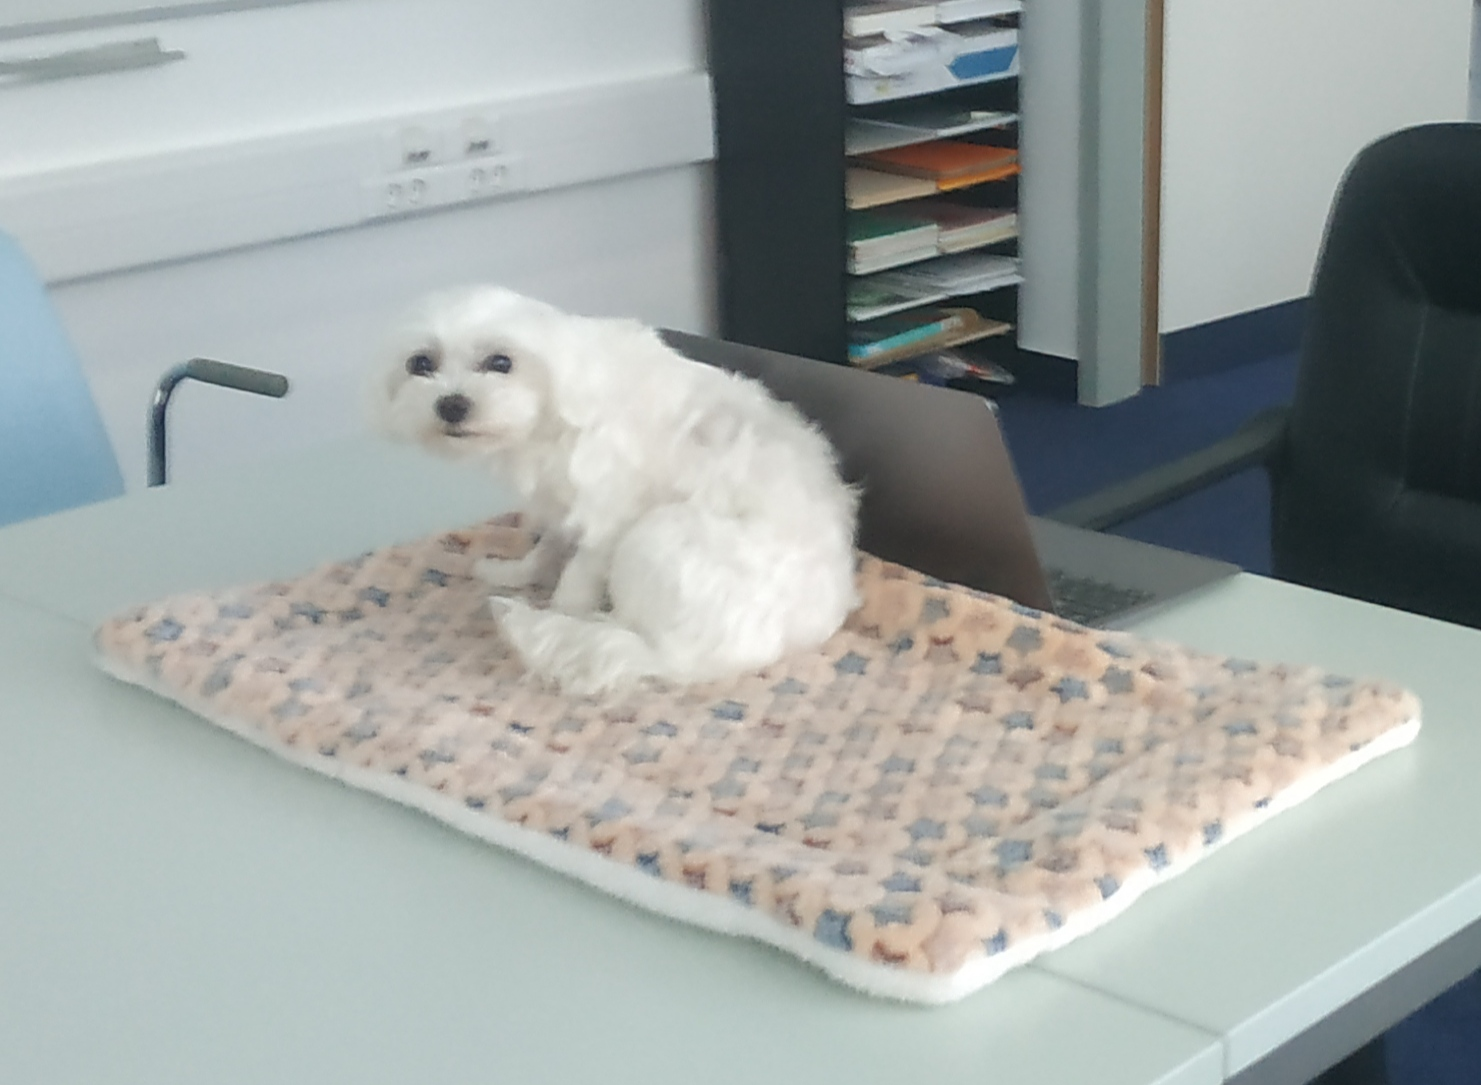
\includegraphics[scale=0.6]{IMG_20221019_165459.jpg}
\end{center}
\caption{Maya is our patronus.}
\end{figure}

Figure Labels: Use 8 point Times New Roman for Figure labels. Use words 
rather than symbols or abbreviations when writing Figure axis labels to 
avoid confusing the reader. As an example, write the quantity 
``Magnetization'', or ``Magnetization, M'', not just ``M''. If including 
units in the label, present them within parentheses. Do not label axes only 
with units. In the example, write ``Magnetization (A/m)'' or ``Magnetization 
\{A[m(1)]\}'', not just ``A/m''. Do not label axes with a ratio of 
quantities and units. For example, write ``Temperature (K)'', not 
``Temperature/K''.

\section*{Acknowledgment}

We would like to say thank you to our research methodology practice teacher Turcsányi-Szabó Márta and lecturer Dr. Horváth Zoltán, who teached us the paper writing methodology and guided us with good good advices.
We are grateful to Eötvös Loránd Tudományegyetem for providing us accessibility to the newest and most prestigious research journals.
This work would not have been possible without the supervision of the bravest and frendliest guard dog Maya, who always encouraged us to work hard.

\section*{References}

Please number citations consecutively within brackets \cite{b1}. The 
sentence punctuation follows the bracket \cite{b2}. Refer simply to the reference 
number, as in \cite{b3}---do not use ``Ref. \cite{b3}'' or ``reference \cite{b3}'' except at 
the beginning of a sentence: ``Reference \cite{b3} was the first $\ldots$''

Number footnotes separately in superscripts. Place the actual footnote at 
the bottom of the column in which it was cited. Do not put footnotes in the 
abstract or reference list. Use letters for table footnotes.

Unless there are six authors or more give all authors' names; do not use 
``et al.''. Papers that have not been published, even if they have been 
submitted for publication, should be cited as ``unpublished'' \cite{b4}. Papers 
that have been accepted for publication should be cited as ``in press'' \cite{b5}. 
Capitalize only the first word in a paper title, except for proper nouns and 
element symbols.

For papers published in translation journals, please give the English 
citation first, followed by the original foreign-language citation \cite{b6}.

\begin{thebibliography}{00}
\bibitem{b1} BUSNATU, Ștefan, et al. Clinical Applications of Artificial Intelligence—An Updated Overview. Journal of Clinical Medicine, 2022, 11.8: 2265.
\bibitem{b2} PFEIL, Juliane, et al. Examination of blood samples using deep learning and mobile microscopy. BMC bioinformatics, 2022, 23.1: 1-14.
\bibitem{b3} HUANG, Qian, et al. Blood cell classification based on hyperspectral imaging with modulated Gabor and CNN. IEEE journal of biomedical and health informatics, 2019, 24.1: 160-170.
\bibitem{b4} BOLDÚ, Laura, et al. A deep learning model (ALNet) for the diagnosis of acute leukaemia lineage using peripheral blood cell images. Computer Methods and Programs in Biomedicine, 2021, 202: 105999.
\bibitem{b5} SHAHZAD, Asim, et al. Categorizing white blood cells by utilizing deep features of proposed 4B-AdditionNet-based CNN network with ant colony optimization. Complex and Intelligent Systems, 2022, 8.4: 3143-3159.
\bibitem{b6} RAHIMZADEH, Mohammad; ATTAR, Abolfazl. A modified deep convolutional neural network for detecting COVID-19 and pneumonia from chest X-ray images based on the concatenation of Xception and ResNet50V2. Informatics in medicine unlocked, 2020, 19: 100360.
\bibitem{b7} KHAN, Siraj, et al. A review on traditional machine learning and deep learning models for WBCs classification in blood smear images. IEEE Access, 2020, 9: 10657-10673.
\end{thebibliography}
\vspace{12pt}
\color{red}
\end{document}

